
\item Line $l$ is the bisector of an angle $\angle{A}$ and $B$ is a point on line $l$. $BP = BQ$ are perpendiculars from $B$ to the arms of $\angle{A}$. 
\begin{enumerate}
\item $\triangle{APB} \cong \triangle{AQB}$
\item $BP = BQ$ or $B$ is equidistant from the arms of $\angle{A}$
\end{enumerate}

\textbf{Construction}\\
The input parameters for the construction are shown in Table 
\begin{figure}[H]
    \begin{center}
     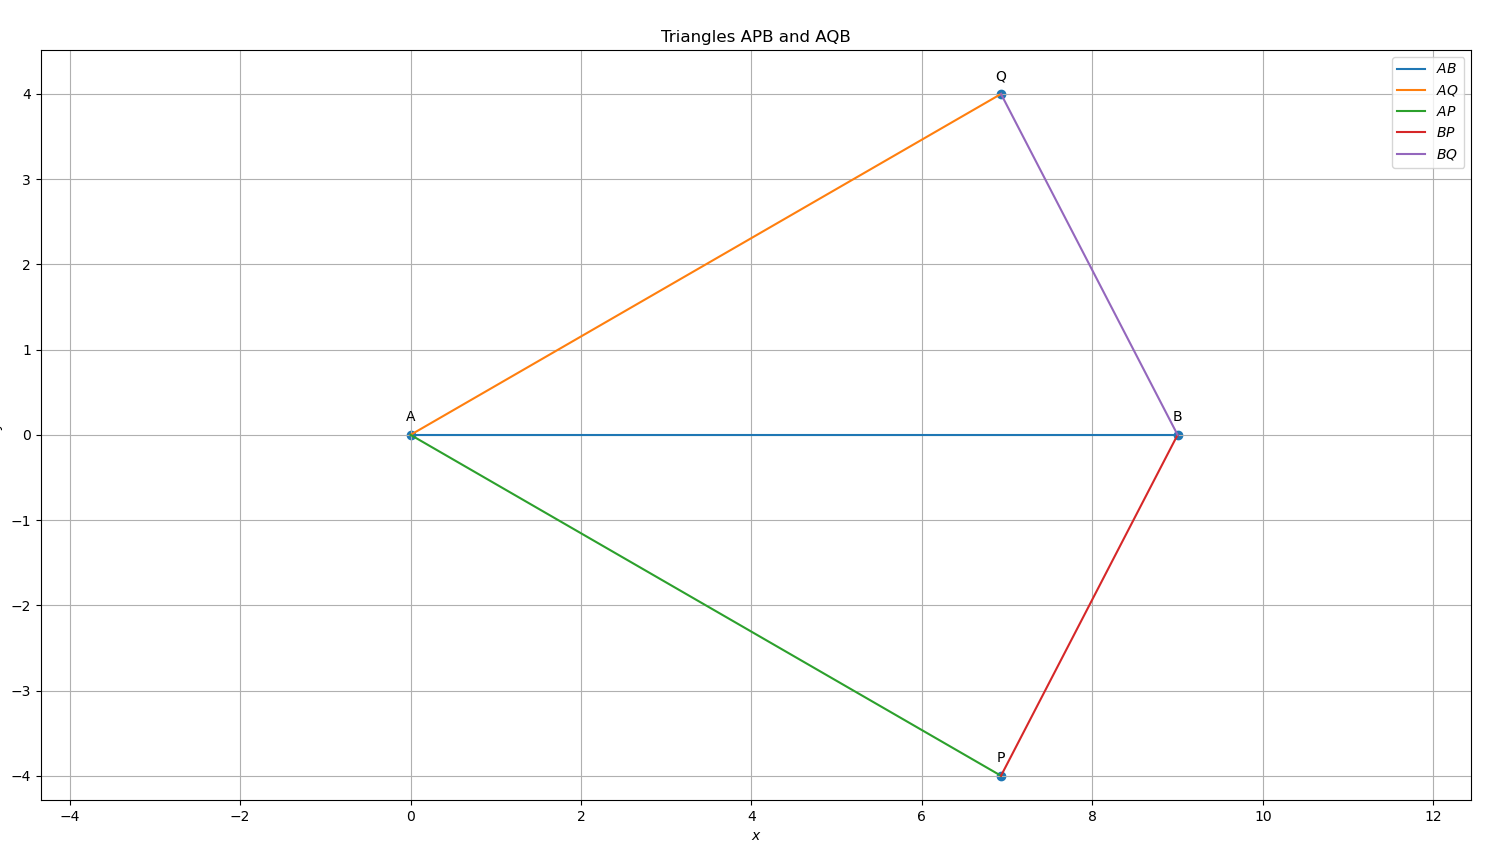
\includegraphics[width=\columnwidth]{chapters/9/7/1/5/figs/tri.png}
    \caption{figure}
    \label{fig:chapters/9/7/1/5/figs/tri.png}   
    \end{center}
\end{figure}

\begin{table}[h]
	  \centering
	  \begin{tabular}{|c|c|p{5cm}|}
\hline
\textbf{Symbol} & \textbf{Value} & \textbf{Description} \\
\hline
$\theta$ & $30\degree$ & $\angle{BAP} = \angle{BAQ}$ \\
\hline
$a$ & $9$ & $AB$ \\
\hline
$c$ & $8$ & $AQ$ \\
\hline
$\vec{e}_1$ & $\myvec{1\\0}$ & Basis vector \\
\hline
\end{tabular}

	  \caption{Parameters}
	  \label{Table}
\end{table}

Let $\vec{A} = \myvec{0\\0}$, $\vec{B} = a\vec{e_1}$, $\vec{Q} = \myvec{c\cos\theta\\c\sin\theta}$, and $\vec{P} = \myvec{c\cos\theta\\-c\sin\theta}$.

